\documentclass[12pt,a4paper,oneside]{book}
\usepackage[italian]{babel}
\usepackage[UTF8]{inputenc}
%\usepackage[latin1]{inputenc}
\usepackage{amsmath}
\usepackage{amsfonts}
\usepackage{amssymb}
\usepackage{graphicx}
\usepackage{eso-pic}
\usepackage{setspace}
\usepackage{fancyhdr} 
\newcommand{\fncyblank}{\fancyhf{}}
\newenvironment{abstract}% 
{\cleardoublepage\fncyblank\null \vfill\begin{center}% 
\bfseries \abstractname \end{center}}% 
{\vfill\null}
\newcommand\AlCentroPagina[1]{% 
\AddToShipoutPicture*{\AtPageCenter{%
\makebox(0,0){\includegraphics%
[width=1\paperwidth]{#1}}}}}
\setlength{\parindent}{0pt}
\setlength{\parskip}{1ex plus 0.5ex minus 0.2ex}
\author{Maria Luisa Feola}
\title{Reti Neurali}

%`` e '': sono le virgolette del TeX; non esistono, nel TeX, le virgolette semplici ( " ) come in Word; le virgolette `` nella tastiera italiana vengono ottenute con la combinazione di tasti “ALT + 96”, mentre le altre sono il segno dell'apostrofo;

% ~ ALT+126 tilde da mettere tra due parole per non farle staccare quando si va a capo

\begin{document}
	%FRONTESPIZIO
	\AlCentroPagina{IMMAGINI/Frontespizio}\thispagestyle{empty}
	
	%DEDICA
	\begin{flushright} 
		\newpage
		\null\vspace{\stretch{1}}
		\thispagestyle{empty}
		\textit{1 $20 \sqrt(e) $ u $<3$ \\
				m$\varepsilon$ 2}
		\vspace{\stretch{2}}\null
	\end{flushright} 
   	%FINE DEDICA
   	%FRASE
   	\begin{flushright} 
   		\newpage
   		\null\vspace{\stretch{1}}
   		\thispagestyle{empty}
   		\textit{Se non puoi passare attraverso una montagna, giraci intorno; \\ se non puoi girarci intorno, passaci sopra;\\ se non puoi passarci sopra, siediti un attimo \\e chiediti se raggiungere l'altro lato sia davvero così importante.\\ \vspace{1cm} Se lo è comincia a scavare una galleria.}
   		\vspace{\stretch{2}}\null
   	\end{flushright} 
   %FINEFRASE
   
   	%INDICE
	\tableofcontents\thispagestyle{empty}
	%FINE INDICE
	
	%INTRODUZIONE
	\chapter*{Introduzione}
	\onehalfspacing
	\addcontentsline{toc}{chapter}{Introduzione}
	prova
	%FINE INTRODUZIONE
		
	%INIZIO DEL PRIMO CAPITOLO
	\chapter{Rete neurale artificiale}
		
		
		
		\section{Cenni storici ed origini}
		Le reti neurali artificiali, dall'inglese \textit{Artificial Neural Network (ANN)}, e la conseguente computazione neurale, sono state costruite ispirandosi ai sistemi neurali biologici, con l'obiettivo di modellarne il comportamento e la struttura e di simularne le funzioni basilari e fondamentali.\\
		Una definizione semplice e formale di tali strutture è fornita dall'inventore del primo neurocomputer, il Dr. Robert Hecht-Nielsen che le definì come: \\
		
		\textit{«...a computing system made up of a number of simple, highly interconnected processing elements, which process information by their dynamic state response to external inputs»}\\
		\textit{(da Neural Network Primer: Parte uno, Maureen Caudill, 1989)}\\
		
		Tradotto in italiano \\
		\textit{«... un sistema di calcolo costituito da una serie di semplici, altamente interconnessi elementi di elaborazione, che elaborano le informazioni attraverso il loro stato dinamico rispondendo agli input esterni.»}\\
		
	    Le basi per lo studio di tali reti furono poste dallo psichiatra Warren McCulloch e del matematico Walter Pitts, i quali riuscirono a riprodurre una rete neurale utilizzando semplici circuiti elettrici collegati tra loro. Questa collaborazione portò alla luce l'analogia che sussiste tra le reti neurali e la macchina di Turing ed in tal modo si capì che qualsiasi operazione eseguita da una rete neurale poteva essere eseguita anche da un computer; infatti le reti che furono prodotte risultavano essere automi a stati finiti in grado di realizzare la logica delle proposizioni e di formulare ipotesi sulla natura dei meccanismi cerebrali, il tutto equivalentemente ad un programma per computer.Il frutto di tale lavoro fu reso noto nel 1943 con la pubblicazione del libro ``\emph{A logical calculus of the ideas immanent in nervous activity}'', nel quale fu schematizzato un combinatore lineare a soglia con dati binari multipli in entrata e un singolo dato binario in uscita.\\
	    Ciò che quindi McCulloch e Pitts riuscirono a fare è presentare un modello di neurone formale dimostrando che reti formate da tali neuroni riuscivano a computare funzioni della logica del primo ordine.\\
	    Un punto di svolta per lo studio delle reti neurali si ebbe successivamente alla pubblicazione del lavoro dello psicologo Donald Hebb, ``\emph{The Organization of Behavior}'' nel 1949.\\
	    Hebb trovò una correlazione tra la psicologia del comportamento umano e la fisiologia del sistema nervoso, donando un grande contributo alla teoria sull'apprendimento associativo, teoria che risultò essere alla base dei metodi di apprendimento delle reti neurali, e che si basava sulla nota legge di Hebb: \textit{«Se un neurone A è abbastanza vicino ad un neurone B da contribuire ripetutamente e in maniera duratura alla sua eccitazione, allora ha luogo in entrambi i neuroni un processo di crescita o di cambiamento metabolico tale per cui l'efficacia di A nell'eccitare B viene accresciuta»}.\\
	    Il decennio che va dagli anni cinquanta agli anni sessanta fu totalmente influenzato dalla legge di Hebb a tal punto che numerosi gruppi di ricerca condussero esperimenti e test sulle funzionalità del cervello, fino a porre le basi per la nascita dell'intelligenza artificiale (AI).\\
	    Nel 1958 Frank Rosenblatt introdusse il primo schema di rete neurale che designò con il termine ``\emph{perceptron}'', in italiano percettrone, allo scopo di fornire un'interpretazione dell'organizzazione generale dei sistemi biologici attraverso un modello mirato all'analisi, in forma matematica, di funzioni quali ad esempio l'immagazzinamento delle informazioni. Il percettrone fu il primo modello di apprendimento supervisionato e presupponeva uno strato di ingresso ed uno di uscita, discriminando gli ingressi in due insiemi linearmente separabili e basandosi su una regola di apprendimento che si appellava alla minimizzazione dell'errore.\\
	    Il percettrone ancora oggi viene utilizzato in varie applicazioni e risultò essere un modello più efficace rispetto a quello binario di McCulloch e Pitts, poichè i suoi pesi sinaptici sono variabili e quindi in grado di apprendere.\\
		Nonostante, però, l'iniziale successo di tale modello e l'interesse mostrato dalla comunità scientifica, tale rete neurale non risultò abbastanza potente; le reti a due strati basate sui percettroni avevano limiti operativi, infatti non riuscivano a risolvere tutte le classi di problemi, in particolare quelli non caratterizzati dalla separabilità lineare delle soluzioni come ad esempio l'operatore \emph{XOR}, ovvero la funzione \emph{OR} esclusivo, che discrimina gli ingressi in modo non linearmente separabile.\\
		Solo negli anni ottanta, con il matematico Paul Werbos, si superarono i limiti del percettrone di Rosenblatt.  Quest'ultimo introdusse uno o più livelli intermedi all'interno delle reti neurali creando una classe chiamata  \emph{Multi-Layers Perceptron}, ovvero percettrone multistrato, il cui metodo di addestramento principale era l'\emph{error backpropagation}, ovvero l'algoritmo di retropropagazione dell'errore, che permetteva la modifica sistematica dei pesi delle connessioni, in modo da rendere la risposta della rete quanto più vicina a quella desiderata.
		Tale algoritmo, proposto nel 1986 da David E.Rumelhart, G. Hinton e R. J. Williams consentì di superare le problematiche legate al percettrone di Rosenblatt e permise di risolvere il problema della separabilità non lineare delle soluzioni, rendendo quindi possibile calcolare la funzione XOR e segnando il definitivo rilancio delle reti neurali.
		
		
		
		\section{Il sistema nervoso e le reti neurali artificiali}
	
		Come accennato nel paragrafo precedente, una rete neurale è un sistema computazionale costruito basandosi sui processi biologici naturali, il cui obiettivo è la riproduzione delle attività tipiche del cervello umano, ad esempio la comprensione del linguaggio, la percezione di immagini, il riconoscimento di forme ecc\dots \\
		In altre parole, lo scopo di una rete neurale artificiale è l’emulazione del sistema nervoso animale, in particolar modo di quello umano, il quale presenta numerose caratteristiche che risultano essere ottime per la riproduzione di un sistema computazionale che lo imiti: è flessibile in quanto si adatta ad ogni tipologia di situazione imparando, è robusto in quanto le cellule nervose muoiono ogni giorno senza avere effetti significativi sulla performance del sistema, è resistente, piccolo e dissipa poca energia. \\
		Tale riproduzione non deve essere intesa come atta alla costruzione di un cervello artificiale. Infatti le caratteristiche delle reti neurali biologiche, riprese dalla computazione neurale artificiale, sono in esigua minoranza: gli stessi neuroni artificiali sono solo un’approssimazione dei neuroni biologici e sono in grado di riprodurre solo tre dei circa centocinquanta processi che sono tipici dei neuroni del cervello umano.\\
		Il sistema nervoso umano può essere pensato, quindi, come una grande struttura computazionale formata da milioni di unità fortemente interconnesse tra loro in modo parallelo e che riesce a trasformare continui input in output ragionevoli. Le reti neurali rappresentano una riproduzione significativa di tale struttura, in particolar modo degli algoritmi di apprendimento e di ottimizzazione, basati su un modello \emph{connessionistico} di calcolo: le operazioni responsabili dello scambio di informazioni avvengono per mezzo dell'interazione tra le unità elementari.
		
		
		
		\section{Il neurone biologico}
		
		Per convincersi a fondo sulla connessione tra le reti neurali artificiali e le reti neurali del sistema nervoso umano, e le numerose analogie che ne derivano, è bene dare una breve illustrazione e descrizione \textbf{(illustrazione e descrizione in questo caso non sono sinonimi?)} del secondo sistema, in modo da far emergere le principali caratteristiche ed i principali costituenti che sono utili al fine della comprensione delle reti neurali.
  		Il sistema nervoso è diviso in tre stadi:
		
		\begin{itemize}
			\item I \emph{recettori}, che convertono gli stimoli esterni in impulsi elettrici che vengono inviati alla rete neurale;
			\item La \emph{rete neurale}, la quale riceve gli impulsi elettrici provenienti dai recettori e li immagazzina come informazioni utili per poter prendere delle decisioni che vengono inviate, anch'esse sotto forma di impulsi elettrici, agli attuatori;
			\item Gli \emph{attuatori} responsabili della trasformazione degli impulsi in risposte per l'ambiente esterno.
		\end{itemize}
	
		
		\begin{figure}[h]
		\centering
		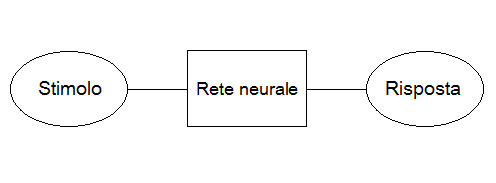
\includegraphics[width=1\linewidth]{IMMAGINI/Sistemanervoso}
		\caption{Stadi del sistema nervoso}
		\label{fig: stadi sistema nervoso}
		\end{figure}
		
		Nel sistema nervoso centrale sono presenti circa $10^{11}$ cellule nervose, i \emph{neuroni}. Tali cellule sono connesse strettamente tra loro attraverso numerosi collegamenti che nel loro insieme vanno a formare la rete neurale. \\
		 Un neurone è formato da un corpo centrale, identificato con il nome di \emph{soma}, all'interno del quale è presente il nucleo, e da molti prolungamenti citoplasmatici, detti \emph{neutriti}, che si distinguono in:
		 
		 \begin{itemize}
		 	\item \emph{dendriti}, organizzati con diramazioni ad albero che costituiscono così il \emph{ramo dendritico};
		 	\item \emph{assone}, la cui parte finale prende il nome di \emph{bottone sinaptico}.
		 \end{itemize}
		 
		 I dendriti ricevono segnali dai neuroni afferenti e li propagano verso il nucleo. L'assone conduce, invece, il segnale verso altre cellule grazie alla presenza del bottone sinaptico alla sua estremità, che risulta essere un'ulteriore ramificazione: quest'ultima va a formare i terminali attraverso i quali i segnali elettrici vengono trasmessi. 
		 
		 \begin{figure}[h]
		 	\centering
		 	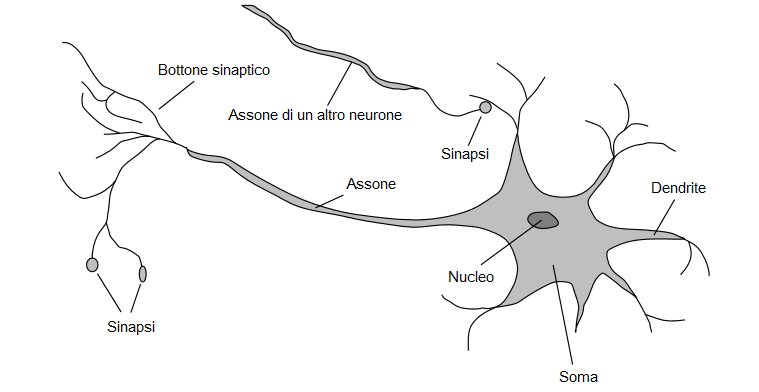
\includegraphics[width=1\linewidth]{IMMAGINI/neuron}
		 	\caption{Neurone biologico}
		 	\label{fig:neuron}
		 \end{figure}
	 
	 	\textbf{Tra un terminale di un assone e la cellula ricevente, esiste uno spazio che viene superato dagli impulsi elettrici per mezzo dei \emph{neurotrasmettitori}, sostanze chimiche che guidano le informazioni tra le cellule e che si suddividono in \emph{eccitatori} se favoriscono la creazione dell'impulso e \emph{soppressori} se inibiscono l'impulso.}\\ Il punto di connessione tra il terminale di un neurone ed il dendrite di un altro costituisce una struttura altamente specializzata che prende il nome di \emph{sinapsi} e che risulta quindi essere la responsabile delle interazioni. La sinapsi svolge due processi: un processo \emph{presinaptico} in cui viene liberato il neurotramettitore ed un processo \emph{postsinaptico}, azionato dal neurotrasmettitore, che rigenera il segnale elettrico.Quindi una sinapsi converte un segnale elettrico in chimico durante il processo postsinaptico per poi riconvertirlo in elettrico durante la postsinapsi.\\ 
	 	Un neurone trasmette un impulso elettrico lungo il suo assone nel momento in cui si verifica una differenza di potenziale elettrico tra l’interno e l’esterno della cellula, provocando la liberazione di un neurotrasmettitore di cui sopra.
		
		
		 
		\section{Modello del neurone artificiale}
		
		La breve illustrazione del sistema neurale umano nel paragrafo precedente suggerisce uno schema per delineare l'organizzazione delle reti neurali artificiali: queste ultime sono formate da un elevato numero di unità computazionali, che possono essere equiparate ai neuroni umani, capaci di eseguire una somma pesata. Tali unità sono collegate tra loro attraverso delle connessioni, così come le sinapsi collegano i neuroni nella rete umana. \\
		Consideriamo una generica unità $j$ costituita da $n$ canali di ingresso:
		
		\begin{center} $x_{1}, x_{2}, ... ,x_{n}$  \end{center}
		
		Gli input provenienti da strati precedenti o direttamente dall'esterno entrano nel neurone tramite tali canali.
		
		\begin{figure}[h]
			\centering
			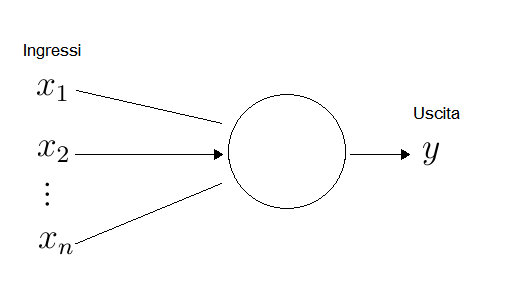
\includegraphics[width=0.7\linewidth]{IMMAGINI/palla1}
			\caption{Canali di ingresso in un neurone}
			\label{fig:palla1}
		\end{figure}
		
		Sulle connessioni sono presenti dei \emph{pesi sinaptici} $w_{i}$, numeri reali che denotano l'\emph{efficacia sinaptica}, ovvero la forza della connessione. Se $w_{i}>0$ il canale è detto \emph{eccitatorio}, se $w_{i}<0$ il canale è \emph{inibitorio}.\\
		I segnali in entrata, pesati dalle rispettive sinapsi, sono convogliati nel \emph{soma} del neurone artificiale, all'interno del quale vengono sommati producendo una combinazione lineare così definita:
		
		\begin{center} $\sum\limits_{i=1}^n w_{i}x_{i}$  \end{center}
		 
		La somma pesata degli ingressi viene indicata con la parola \emph{net} ed il segnale con cui il neurone trasmette la sua attività all'esterno è calcolato applicando una \emph{funzione di attivazione} $\varphi$ che limita l'ampiezza dell'output; si assume per comodità che le ampiezze degli output appartengono all'intervallo $[0,1]$ oppure $[-1,1]$.
		
		\begin{figure}[h]
			\centering
			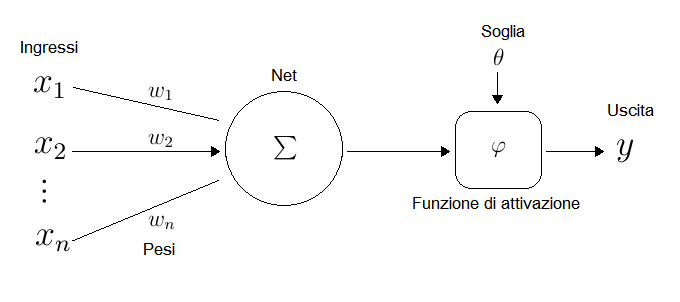
\includegraphics[width=1\linewidth]{IMMAGINI/palla2}
			\caption{Modello neurone}
			\label{fig:palla2}
		\end{figure}
	
		Il modello neuronale include anche un valore \emph{soglia} che ha l'effetto, a seconda della sua positività o negatività, di aumentare o diminuire il valore in ingresso alla funzione di attivazione.\\
		L'output finale sarà allora:
		\begin{center} $y= \varphi (\sum\limits_{i=1}^n w_{i}x_{i})$  \end{center}
	
		\clearpage
		E se indichiamo con $\theta$ il valore di soglia, si avrà:
		\begin{center} $y= \varphi (\sum\limits_{i=1}^n w_{i}x_{i}-\theta)$  \end{center}
		
		Interpretando la soglia come il peso associato ad un ulteriore canale di ingresso $x_{0}$, e quindi $w_{0}=\theta$, potremmo anche scrivere : 
		\begin{center} $y= \varphi (\sum\limits_{i=0}^n w_{i}x_{i})$  \end{center}
		Il modello finale sarà:
		
		\begin{figure}[h]
			\centering
			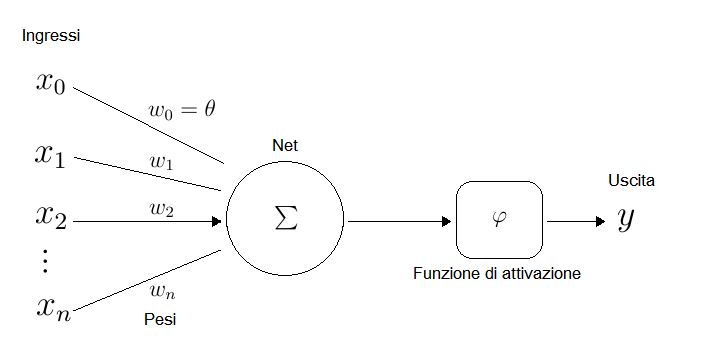
\includegraphics[width=1\linewidth]{IMMAGINI/palla3}
			\caption{Modello neurone con soglia}
			\label{fig:palla3}
		\end{figure}
		
		L'effetto di un segnale $ x_{i} $ sul neurone è quindi uguale al prodotto 
		$w_{i}$ $\cdot$ $x_{i}$ dove $w_{i}$ è il peso attribuito alla sinapsi corrispondente ed il potenziale di attivazione è dato dalla somma algebrica dei prodotti di tutti i segnali di ingresso e dei valori dei pesi corrispondenti.\\
	 	Schematizzando, ed individuando il neurone artificiale come l'unità di calcolo fondamentale della rete neurale, gli elementi base che lo rappresentano sono:
		\begin{itemize}
			\item Un insieme di connessioni;
			\item Un sommatore;
			\item Una funzione di attivazione;
			\item Un valore di soglia.
		\end{itemize}
		
		\section{Funzioni di attivazione}
		
		
		Discorso scritto da me che mi piace e che devo introdurre in questo paragrafo!\\
		io) Abbiamo a che fare quindi con sistemi altamente paralleli ed addestrabili il cui apprendimento avviene attraverso la modifica dei pesi delle connessioni. Sono inoltre sistemi tolleranti agli errori con la capacità di produrre output ragionevoli con input mai incontrati prima durante l'apprendimento. \textbf{Perchè addestrabili?} L'attività della singola unità è semplice e la potenza dipende dalla configurazione delle connessioni.
		Partendo dalle unità di input, a cui vengono forniti i dati dei problema da risolvere, la computazione si propaga in parallelo nella rete fino alle unità di output che forniscono il risultato.
		Il tratto peculiare delle reti neurali è che queste vengono addestrate utilizzando algoritmi di apprendimento mediante una serie di esempi della realtà da modellare.
		
	%FINE DEL PRIMO CAPITOLO
	
	\chapter{Feed Forward}
	\chapter{Ricorrenti}

\clearpage 
%\phantomsection 
\begin{thebibliography}{9} 
	\addcontentsline{toc}{chapter}{\refname}
	\bibitem[1]{Lazzarini} Prof.ssa Lazzarini Beatrice, (2015), \emph{Introduzione alle reti neurali.}
	\bibitem[2]{Gambosi} Prof. Gambosi Giorgio, (2010), \emph{Reti neurali, note dal corso di Machine Learning.}
	\bibitem[3]{Labonia} Prof.ssa Labonia Laura, \emph{Storia delle reti neurali artificiali.}
	\bibitem[4]{Bicego} Prof. Bicego Manuele, \emph{Riconoscimento e recupero dell’informazione per bioinformatica. Reti neurali.}
	\bibitem[5]{Pioggia} Ing. Pioggia Giovanni, (2009), \emph{Modelli di sistemi fisiologici}
 \end{thebibliography}
	
\end{document}